\documentclass[sigconf]{acmart}

\settopmatter{printacmref=true}
\renewcommand\footnotetextcopyrightpermission[1]{}
\pagestyle{plain}


% Packages
\usepackage{times}
\usepackage{geometry}
\usepackage{amsmath}
\usepackage{listings}
% \usepackage[hyphens]{url}
\usepackage{hyperref}
\usepackage{pgfplots}
\usepackage[utf8]{inputenc}

\setlength{\headheight}{15.62192pt}
\addtolength{\topmargin}{-2.62192pt}
\begin{document}

\title{Analyzing the Impact of Automatic Dependency Management in Serverless Computing}
\author{Richard Paul}
\affiliation{%
	\institution{University of Massachusetts Amherst}
	\city{Amherst}
	\state{MA}
	\country{USA}
}
\email{rdpaul@umass.edu}

\begin{abstract}
	As cloud computing evolves, serverless architectures have gained significant traction due to their scalability, cost-effectiveness, and ease of deployment. However, the automation of dependency management within serverless environments introduces unique security challenges that need examining. This paper presents a comprehensive examination of automatic dependency management in serverless computing from a security perspective. By evaluating common serverless applications, we can identify prevalent methods and tools for managing dependencies, focusing on their security implications. This study delves into the mechanisms of popular dependency management programs, such as Snyk and Dependabot, to assess their effectiveness in mitigating vulnerabilities. Additionally, an online survey of developers provides insights into real-world practices and perceptions regarding dependency management in serverless contexts. Our findings highlight specific security risks, best practices, and potential improvements, including enhanced vulnerability scanning, better transparency in automated updates, and developer education to bolster the security of serverless applications. 
\end{abstract}

\begin{CCSXML}
	<ccs2012>
	<concept>
	<concept_id>10002978.10003006.10003007</concept_id>
	<concept_desc>Security and privacy~Operating systems security</concept_desc>
	<concept_significance>500</concept_significance>
	</concept>
	<concept>
	<concept_id>10010520.10010575</concept_id>
	<concept_desc>Computer systems organization~Cloud computing</concept_desc>
	<concept_significance>300</concept_significance>
	</concept>
	<concept>
	<concept_id>10010520.10010553</concept_id>
	<concept_desc>Computer systems organization~Embedded systems</concept_desc>
	<concept_significance>100</concept_significance>
	</concept>
	</ccs2012>
\end{CCSXML}

\ccsdesc[500]{Security and privacy~Operating systems security}
\ccsdesc[300]{Computer systems organization~Cloud computing}
\ccsdesc[100]{Computer systems organization~Embedded systems}

\keywords{Serverless computing, dependency management, large-scale systems, security, cloud computing}

\maketitle

\acmConference[690G Final Project Report]{Large Scale System Security, Spring 2024}{University of Massachusetts Amherst}

\section{Introduction}
As cloud computing evolves, serverless architectures have emerged as a paradigm shift, allowing developers to build and deploy applications without the costly overhead of managing servers. This allows developers to abstract away the infrastructure, focusing on code and functionality. However, this introduces new challenges, including in the realm of security \cite{baldini2017serverless}. One important concern is dependency management. Dependencies, or external libraries and packages for an application, can contain vulnerabilities that pose security risks \cite{marin2022serverless}. Recognizing this issue, some serverless cloud providers have begun to integrate automatic dependency vulnerability checking and updating. This paper aims to scrutinize the benefits and drawbacks of those features, to provide a detailed analysis of their impact on serverless computing.

The introduction of automatic dependency vulnerability checking and updating is seen as a benefit for the security of serverless applications. By incessantly scanning for and remedying known vulnerabilities within dependencies, cloud providers can curb the likelihood of security breaches \cite{snyk2023security}. This preventive measure can bolster application security and alleviate developers from the cumbersome task of manually tracking and updating their dependencies. As Buckholz notes, this can align with the philosophy of serverless development by allowing developers to focus more on innovation than maintenance \cite{buckholz2018serverless}.

However, this innovation has its limitations. The automatic alteration of dependencies can lead to unintended changes or incompatibilities, which will potentially compromise application performance \cite{benischke2023updates}. Additionally, the lack of transparency in automatic dependency checking could result in a diminished understanding and oversight of faults in the application. It may also force developers to rely upon a certain cloud provider to maintain the dependencies, leading to vendor lock-in \cite{kavis2014cloud}.
Furthermore, the thoroughness and reliability of automated vulnerability checks is still in question, and may lead some developers to believe their application is protected when it still contains security vulnerabilities.

\section{Background}
Serverless computing has dramatically changed the landscape of cloud services, offering a new paradigm for application deployment and management. Serverless computing allows code to execute in response to events without the need for provisioning or managing individual servers. This abstracts away the infrastructure layer, significantly simplifying the administrative responsibilities upon application developers \cite{roberts2020lambda}. This model, predominantly offered through Functions-as-a-Service (FaaS) platforms like AWS Lambda, Azure Functions, and Google Cloud Functions, allows developer to focus on code that contributes directly to their application, rather than on the underlying operational complexities \cite{villamizar2015evaluating}.

A critical aspect of developing in a serverless environment is the management of dependencies, external libraries or packages that an application uses to perform functions. Dependencies can include many things from frameworks for web applications to libraries for accessing cloud services. Dependency management is not a trivial task, they must be kept up-to-date to incorporate bug fixes, new features, and, most importantly, security updates \cite{benischke2023updates}. The National Vulnerability Database, a U.S. government repository of vulnerability management data, has shown an increasing amount of vulnerabilities among common dependencies, underscoring the importance of well-thought-out dependency management \cite{NVDdatabase}.

This has led to rise in automatic dependency checking and updating software to help manage these dependency issues. Tools like Snyk, Dependabot, and Renovate can automate the process of detecting vulnerabilities in a projects dependencies and automatically update those dependencies to a new secure version. This is vital in a serverless environment where the agility and scalability of application can be compromised by vulnerable dependencies \cite{estrin2021handbook}.

However, the implementation of automatic dependency management in serverless computing still has significant challenges. The automated update process must be carefully managed to ensure that updates do not introduce changes that break the application. In addition, reliance on automated tools can lead to a decreased understanding of dependency management among developers, potentially leading to complacency and increased security risks when automated systems fail \cite{hilton2016ci}.

The security risk in dependencies primarily come from two distinct factors: the external nature of the dependencies and the complex and opaque dependency trees that they can form. A single application may directly depend on hundreds of external libraries, which may themselves depend on thousands more. This complexity significantly increases the attack surface of the applications, as each external dependency is a point of failure for attackers \cite{OWASP2021top}. For example, there was a notable incident where a popular NPM package, event-stream, was compromised to steal cryptocurrency for the attackers, showcasing the cascading risk a single vulnerable dependency poses to thousands of different applications \cite{fox2018open}.

Moreover, the ephemeral and stateless nature of serverless function can significantly increase these risks. Since serverless applications scale dynamically with the resources demanded from them, a vulnerability in a single dependency can rapidly propagate across multiple instances, amplifying the potential impact of any security branch \cite{kavis2014cloud}.

To counteract these risks, there exists several notable mitigation strategies and best practices that have been recommended and adopted:
\begin{itemize}
	\item Implementing regular vulnerability scanning and dependency review. Using tools like Snyk and OWASP Dependency-Check can provide automated vulnerability scanning and are important to ensure a robust security management.
	\item The 'Shift-Left' security approach, which argues that security needs to be a focus from the start of development, or else you will end up chasing your tail after the vulnerabilities that will almost certainly exist.
	\item Principle of Least Privilege (PoLP) is a foundational security principal to ensure that programs only have access to the permissions they need. This can be implemented with dependencies to help box them in and not give them undue access.
	\item Use versions of dependencies that have been thoroughly vetted. This can avoid new vulnerabilities that could come up in new versions, but may delay the ability for your application to use new features/ get updates to old unseen vulnerabilities.
	\item Developer education has been cited as a very important part of dependency management. Ultimately, the buck stops with the development team, and it's vital to insure all developers are cognizant of the risks involved with using dependencies, and best practices for doing so.
\end{itemize}

\section{Comparative Analysis of Serverless Platforms}

\subsection{AWS Lambda}

\subsubsection{Dependency Management Tools and Integrations}

AWS Lambda provides robust integration with various dependency management tools, offering comprehensive support for automated vulnerability scanning and updates. Key integrations include:

\begin{itemize}
    \item \textbf{AWS CodePipeline and CodeBuild:} These services automate the process of building, testing, and deploying Lambda functions. They support integration with third-party tools like Snyk and Dependabot, which facilitate the detection and updating of vulnerable dependencies. This integration ensures that dependencies are continuously monitored and updated, reducing the risk of security vulnerabilities \cite{awsCI2023}.
    \item \textbf{AWS SAM (Serverless Application Model):} The AWS SAM CLI aids in managing dependencies for Lambda functions. It allows developers to define and build serverless applications using AWS resources. The SAM CLI also supports local testing and deployment, providing a seamless workflow for managing dependencies during development \cite{awssam2023}.
\end{itemize}

\subsubsection{Security Features}

AWS Lambda incorporates several security features designed to manage dependencies securely:

\begin{itemize}
    \item \textbf{Snyk Integration:} AWS CodePipeline can integrate with Snyk to continuously monitor for vulnerabilities in dependencies and provide automated fixes. This integration helps ensure that serverless applications remain secure over time by addressing known vulnerabilities promptly \cite{snykaws2023}.
    \item \textbf{AWS IAM and Secrets Manager:} These services manage permissions and sensitive information, ensuring that Lambda functions and their dependencies are secure. AWS IAM provides fine-grained access control, while Secrets Manager enables secure handling of sensitive data such as API keys and database credentials \cite{awsSecurity2023}.
    \item \textbf{Amazon Inspector:} This service provides automated security assessments to help improve the security and compliance of applications deployed on AWS, including Lambda functions. Amazon Inspector identifies potential security issues and vulnerabilities in dependencies, offering actionable insights to enhance the security posture of serverless applications \cite{awsinspector2023}.
\end{itemize}

\subsubsection{User Experience and Documentation}

AWS Lambda offers extensive documentation and a large community of users, providing a wealth of resources for developers. The AWS Well-Architected Framework offers best practices and guidelines, particularly for security and dependency management. The Lambda console and SAM CLI provide intuitive interfaces for managing and deploying functions, making it easier for developers to implement best practices and manage dependencies effectively \cite{awsWell2023}.

\subsubsection{Performance Impact}

The impact of automatic dependency updates on AWS Lambda's performance is generally minimal. However, some users have reported issues with compatibility and stability following updates. AWS CloudWatch offers detailed monitoring and logging to help identify and resolve performance issues related to dependency management. Continuous monitoring ensures that any negative impacts on performance are quickly addressed, maintaining the reliability of serverless applications \cite{lambdaPerformance2023}.

\subsection{Azure Functions}

\subsubsection{Dependency Management Tools and Integrations}

Azure Functions supports several tools and services for managing dependencies:

\begin{itemize}
    \item \textbf{Azure DevOps:} Azure DevOps offers comprehensive CI/CD pipelines with built-in capabilities for managing dependencies. It supports integration with tools like Renovate and Dependabot for automated vulnerability detection and updates. This integration allows developers to maintain secure and up-to-date dependencies with minimal manual effort \cite{azureDevOps2023}.
    \item \textbf{Azure Functions Core Tools:} These tools facilitate local development and testing, including dependency management through NuGet (for .NET) and npm (for Node.js). The Azure Functions Core Tools provide a seamless experience for managing dependencies during the development phase \cite{azureCoreTools2023}.
\end{itemize}

\subsubsection{Security Features}

Azure Functions provides a range of security features related to dependency management:

\begin{itemize}
    \item \textbf{OWASP Dependency-Check Integration:} Azure Pipelines can be configured to use OWASP Dependency-Check to identify and fix vulnerabilities in dependencies. This integration enhances the security of serverless applications by ensuring that dependencies are continuously monitored for known vulnerabilities \cite{azureowasp2023}.
    \item \textbf{Azure Security Center and Key Vault:} These services help manage secrets and credentials securely. Azure Security Center provides advanced threat protection for Azure resources, while Key Vault ensures that sensitive information is handled securely \cite{azureSecurity2023}.
    \item \textbf{Managed Identities:} Managed Identities provide secure and automatic management of service principal identities for applications running in Azure. This feature helps to reduce the complexity and security risks associated with managing credentials manually \cite{azureManagedIdentities2023}.
\end{itemize}

\subsubsection{User Experience and Documentation}

Azure Functions is supported by detailed documentation available through Microsoft Learn. This includes tutorials, best practices, and case studies that help developers implement and manage dependency management practices effectively. The platform's integration with the broader Azure ecosystem provides a seamless experience for managing serverless applications \cite{azureLearn2023}.

\subsubsection{Performance Impact}

Performance and stability are generally reliable on Azure Functions. The platform's robust monitoring tools, such as Azure Monitor and Application Insights, provide comprehensive insights into application performance. These tools help developers quickly address any issues that arise from automatic dependency updates, ensuring the smooth operation of serverless applications \cite{azurePerformance2023}.

\subsection{Google Cloud Functions}

\subsubsection{Dependency Management Tools and Integrations}

Google Cloud Functions supports several dependency management tools and integrations:

\begin{itemize}
    \item \textbf{Google Cloud Build:} This service integrates with dependency management tools like OWASP Dependency-Check for automated vulnerability scanning and updating. Google Cloud Build provides a seamless CI/CD pipeline that helps maintain secure and up-to-date dependencies \cite{googleBuild2023}.
    \item \textbf{Third-Party Tools:} Google Cloud Functions also supports integration with tools like Snyk and Dependabot, allowing developers to automate the detection and remediation of vulnerable dependencies. These integrations ensure continuous monitoring and prompt updates of dependencies \cite{googlesnyk2023}.
\end{itemize}

\subsubsection{Security Features}

Google Cloud Functions includes several security features designed to manage dependencies securely:

\begin{itemize}
    \item \textbf{Google Cloud IAM and Secret Manager:} These services manage permissions and sensitive data, ensuring that dependencies are handled securely. Google Cloud IAM provides detailed access control, while Secret Manager securely stores and manages access to sensitive information \cite{googleSecurity2023}.
    \item \textbf{Google Cloud Armor:} This service provides protection against web threats and DDoS attacks, enhancing the security of serverless applications. Cloud Armor helps mitigate risks associated with exposed dependencies \cite{googleArmor2023}.
    \item \textbf{Security Command Center:} Offers a centralized view of security across Google Cloud resources, including automated vulnerability scanning and monitoring. This tool helps identify and mitigate security risks in dependencies \cite{googleSCC2023}.
\end{itemize}

\subsubsection{User Experience and Documentation}

Google Cloud Functions is known for its user-friendly interface and comprehensive documentation. The platform's documentation portal provides detailed guides, best practices, and examples, making it accessible for developers of all skill levels. The integration with Google Cloud Console offers a seamless experience for managing serverless applications and their dependencies \cite{googleDocs2023}.

\subsubsection{Performance Impact}

Performance and reliability are strong points for Google Cloud Functions. Users report minimal issues related to automatic dependency updates. Google Cloud's monitoring tools, such as Google Cloud Operations Suite (formerly Stackdriver), provide detailed insights into application performance, helping developers quickly identify and resolve issues. These tools ensure that automatic updates do not negatively impact the performance of serverless applications \cite{googlePerformance2023}.

\subsection{Comparison and Analysis}

\begin{figure*}[ht]
	\centering
	\begin{tabular}{|p{4cm}|p{4cm}|p{4cm}|p{4cm}|}
	\hline
	\textbf{Feature} & \textbf{AWS Lambda} & \textbf{Google Cloud Functions} & \textbf{Azure Functions} \\
	\hline
	\textbf{Dependency Management} & 
	Dependencies are packaged with the deployment package. Lambda Layers can be used to manage shared code and libraries. & 
	Dependencies are included in the project folder or specified in a \texttt{requirements.txt} or \texttt{package.json}. & 
	Dependencies are included directly in the code or via a \texttt{requirements.txt} or \texttt{project.json}. Also supports NuGet packages. \\
	\hline
	\textbf{Automatic Dependency Updates} & 
	Supports automatic updates through integration with tools like Snyk and Dependabot via CodePipeline and CodeBuild. & 
	Supports automatic dependency resolution and updates through integration with tools like Snyk and Dependabot via Cloud Build. & 
	Supports automatic dependency management through Azure DevOps, including tools like Renovate and Dependabot. \\
	\hline
	\textbf{Security Features} & 
	AWS IAM for fine-grained access control, Secrets Manager for sensitive data, Amazon Inspector for security assessments, Snyk for vulnerability scanning. & 
	Google Cloud IAM for detailed access control, Secret Manager for managing sensitive data, Cloud Armor for threat protection, Security Command Center for centralized security monitoring. & 
	Azure Security Center for advanced threat protection, Key Vault for secrets management, Managed Identities for secure identity management, OWASP Dependency-Check for vulnerability scanning. \\
	\hline
	\textbf{User Experience and Documentation} & 
	Extensive documentation, AWS Well-Architected Framework for best practices, large community support. & 
	User-friendly interface, comprehensive documentation portal with detailed guides and examples, seamless integration with Google Cloud Console. & 
	Detailed documentation via Microsoft Learn, including tutorials, best practices, and case studies, integrated development environment support. \\
	\hline
	\textbf{Performance Impact} & 
	Minimal, with detailed monitoring and logging via AWS CloudWatch. Some users report occasional compatibility and stability issues post updates. & 
	Minimal, with robust monitoring tools like Google Cloud Operations Suite (formerly Stackdriver) ensuring minimal performance disruption. & 
	Generally reliable, with comprehensive insights into application performance provided by Azure Monitor and Application Insights. \\
	\hline
	\textbf{Supported Languages} & 
	Node.js, Python, Ruby, Java, Go, .NET Core, and custom runtimes. & 
	Node.js, Python, Go, Java, .NET, Ruby, PHP, and more. & 
	C\#, F\#, Java, JavaScript (Node.js), Python, TypeScript, PowerShell. \\
	\hline
	\textbf{Environment and Runtime} & 
	Provides a runtime environment with custom runtime support via the Runtime API. & 
	Managed runtime environment with limited customization. & 
	Highly customizable environment with support for different OS and runtime versions. \\
	\hline
	\textbf{Version Management} & 
	Supports versioning and aliasing for managing different deployment stages. & 
	Uses Cloud Source Repositories for version control; does not natively handle multiple versions of a function. & 
	Supports multiple versions and deployment slots for staging and production environments. \\
	\hline
	\end{tabular}
	\caption{Comparison of AWS Lambda, Google Cloud Functions, and Azure Functions from an Automatic Dependency Management and Security Perspective}
	\label{fig:comparison}
	\end{figure*}
	

\subsubsection{Dependency Management Tools and Integrations}

All three platforms, AWS Lambda, Azure Functions, and Google Cloud Functions, provide robust integrations with various dependency management tools. AWS Lambda and Azure Functions both support integration with third-party tools like Snyk and Dependabot, facilitating automated vulnerability detection and updates \cite{awsCI2023, azureDevOps2023, googlesnyk2023}. Google Cloud Functions integrates with Google Cloud Build and supports third-party tools like Snyk, ensuring continuous monitoring and prompt updates \cite{googleBuild2023}.

\begin{itemize}
    \item \textbf{AWS Lambda:} Offers integration with AWS CodePipeline and CodeBuild for CI/CD, along with AWS SAM CLI for managing dependencies during development \cite{awsCI2023, awssam2023}.
    \item \textbf{Azure Functions:} Provides comprehensive CI/CD pipelines through Azure DevOps and supports dependency management through Azure Functions Core Tools \cite{azureDevOps2023, azureCoreTools2023}.
    \item \textbf{Google Cloud Functions:} Integrates with Google Cloud Build and supports third-party tools like Snyk and Dependabot for automated vulnerability management \cite{googleBuild2023, googlesnyk2023}.
\end{itemize}

\subsubsection{Security Features}

Each platform offers a range of security features aimed at managing dependencies securely:

\begin{itemize}
    \item \textbf{AWS Lambda:} Utilizes services like AWS IAM, Secrets Manager, and Amazon Inspector to enhance the security of dependencies \cite{awsSecurity2023, awsinspector2023}.
    \item \textbf{Azure Functions:} Incorporates Azure Security Center, Key Vault, and Managed Identities to ensure secure handling of dependencies \cite{azureSecurity2023, azureManagedIdentities2023}.
    \item \textbf{Google Cloud Functions:} Provides security features through Google Cloud IAM, Secret Manager, Cloud Armor, and Security Command Center \cite{googleSecurity2023, googleArmor2023, googleSCC2023}.
\end{itemize}

\subsubsection{User Experience and Documentation}

All three platforms are known for their comprehensive documentation and user-friendly interfaces, which help developers implement and manage dependency management practices effectively:

\begin{itemize}
    \item \textbf{AWS Lambda:} Offers extensive documentation and a large community of users, with tools like the AWS Well-Architected Framework providing best practices \cite{awsWell2023}.
    \item \textbf{Azure Functions:} Supported by detailed documentation available through Microsoft Learn, including tutorials and best practices \cite{azureLearn2023}.
    \item \textbf{Google Cloud Functions:} Known for its user-friendly interface and comprehensive documentation portal, providing detailed guides and examples \cite{googleDocs2023}.
\end{itemize}

\subsubsection{Performance Impact}

The performance impact of automatic dependency updates is generally minimal across all three platforms, though some users have reported occasional issues with compatibility and stability:

\begin{itemize}
    \item \textbf{AWS Lambda:} Uses AWS CloudWatch for detailed monitoring and logging, helping to identify and resolve performance issues related to dependency management \cite{lambdaPerformance2023}.
    \item \textbf{Azure Functions:} Relies on robust monitoring tools like Azure Monitor and Application Insights to provide comprehensive insights into application performance \cite{azurePerformance2023}.
    \item \textbf{Google Cloud Functions:} Employs Google Cloud Operations Suite for detailed insights into application performance, ensuring minimal disruption from automatic updates \cite{googlePerformance2023}.
\end{itemize}

\subsubsection{Summary of Findings}

Our evaluation reveals that each platform offers distinct strengths in dependency management:

\begin{itemize}
    \item \textbf{AWS Lambda:} Provides extensive integration with dependency management tools and strong security features. Its comprehensive documentation and large community support make it a robust choice for developers, although occasional performance issues may arise from automatic updates.
    \item \textbf{Azure Functions:} Offers enterprise-grade support and security features, with a steep learning curve but strong performance and reliability. Its integration with Azure DevOps and security tools like OWASP Dependency-Check make it a powerful option for managing dependencies.
    \item \textbf{Google Cloud Functions:} Known for ease of use and comprehensive documentation. Its strong performance and security features, along with seamless integration with Google Cloud tools, make it a reliable choice for developers looking for user-friendly dependency management solutions.
\end{itemize}

Overall, the choice of platform depends on specific organizational needs and developer preferences. AWS Lambda stands out for its robust ecosystem and community support, Azure Functions excels in enterprise-grade features and security, and Google Cloud Functions offers a user-friendly experience with strong performance and security features.


\section{Snyk and Dependabot in Serverless Environments}

Dependency management tools like Snyk and Dependabot play a critical role in maintaining the security and functionality of serverless applications. These tools automate the detection and remediation of vulnerabilities in dependencies, helping developers manage the complexities associated with third-party libraries and packages.

Snyk is a popular tool designed to find and fix vulnerabilities in dependencies. It integrates with various CI/CD pipelines and development tools, providing continuous security monitoring and automated fixes. Snyk continuously scans for vulnerabilities in dependencies and offers detailed reports on potential security risks, enabling developers to address these issues promptly. One of the key features of Snyk is its ability to automatically fix vulnerabilities by suggesting or applying updates to secure versions of dependencies. This capability reduces the manual effort required to manage dependencies, allowing developers to focus on core application logic. Snyk integrates seamlessly with CI/CD pipelines, such as Jenkins, GitHub Actions, and GitLab CI, enabling automated security checks during the build and deployment process. Additionally, Snyk integrates with popular IDEs like Visual Studio Code and IntelliJ IDEA, providing real-time vulnerability detection during development \cite{snyk2023, snykIDE2023}.

The upsides of using Snyk include continuous security monitoring, which ensures that applications remain secure over time, and automated fixes that reduce the manual effort required to manage dependencies. Snyk also provides comprehensive reports that help developers understand the impact and severity of identified issues, and it has a strong community and extensive documentation that offer valuable resources for developers. However, there are some downsides. Automatic updates may introduce compatibility issues, especially if new versions of dependencies have breaking changes \cite{benischke2023updates}. Continuous scanning can also introduce performance overhead, potentially affecting build times and deployment speed. Additionally, Snyk may sometimes flag vulnerabilities that do not pose significant risks, leading to unnecessary updates or fixes \cite{snykFalsePositives2023}.

Dependabot, a GitHub-native tool, automates dependency updates by creating pull requests to update dependencies to the latest versions, helping to maintain secure and up-to-date projects. Dependabot automatically checks for outdated dependencies and creates pull requests to update them, integrating seamlessly with GitHub Security Alerts to notify developers of vulnerabilities in their dependencies. Developers can configure Dependabot to update dependencies according to their preferred schedule and update policies. Dependabot also works well with CI/CD tools, facilitating automated testing and deployment of updated dependencies \cite{dependabot2023}.

The primary benefits of Dependabot include its ease of use and the automation of pull requests, which simplify the process of updating dependencies and reduce manual effort and potential human error. Its integration with GitHub Security Alerts ensures that developers are promptly informed of vulnerabilities. Furthermore, Dependabot's customization options allow developers to tailor update schedules and policies to fit their project needs, providing flexibility in dependency management. However, there are some downsides to using Dependabot. Automated pull requests can lead to merge conflicts, especially in projects with complex dependency trees. Frequent updates and pull requests can consume resources and overwhelm development teams, particularly in large projects. Moreover, Dependabot's functionality is primarily focused on GitHub-hosted projects, limiting its use for projects hosted on other platforms.

In serverless environments, where applications are highly modular and rely heavily on third-party libraries, tools like Snyk and Dependabot offer significant advantages. They improve security by ensuring that serverless applications remain secure through automated vulnerability detection and updates, reducing the risk of exploitation. Automation of dependency management tasks also allows developers to focus on building and optimizing serverless functions, enhancing productivity. Additionally, automated tools can handle the scale and complexity of serverless applications, where dependencies may be numerous and frequently updated.

However, there are potential downsides to using these tools in serverless environments. Automatic updates can introduce compatibility issues, which may be challenging to debug due to the distributed nature of serverless functions \cite{benischke2023updates}. Continuous scanning and frequent updates can introduce performance overhead, affecting the deployment speed and runtime performance of serverless applications. Finally, dependence on external tools for security and updates may lead to vendor lock-in and reduced control over the dependency management process \cite{kavis2014cloud}.

Overall, while tools like Snyk and Dependabot provide valuable automation and security benefits in serverless environments, developers must carefully manage potential downsides to ensure application stability and performance.

\section{Language-Based Package Managers}

Language-based package managers, such as Maven for Java, npm for Node.js, and pip for Python, play a crucial role in managing dependencies within serverless applications. These package managers automate the process of installing, updating, and managing libraries and frameworks that applications rely on. However, the integration of these package managers with security tools like Snyk and Dependabot, as well as Continuous Integration/Continuous Deployment (CI/CD) systems, is essential for maintaining the security and integrity of serverless applications.

\subsection{Role of Language-Based Package Managers}

Language-based package managers simplify dependency management by providing a standardized way to declare, install, and update dependencies. For example:
\begin{itemize}
    \item \textbf{Maven:} Utilized primarily in Java projects, Maven uses a \texttt{pom.xml} file to manage project dependencies, plugins, and build configurations.
    \item \textbf{npm:} Commonly used in Node.js projects, npm uses a \texttt{package} \texttt{.json} file to manage dependencies and scripts for building and running applications.
    \item \textbf{pip:} Used for Python projects, pip installs and manages packages listed in a \texttt{requirements.txt} file.
\end{itemize}
These package managers streamline the development process by automating dependency resolution and ensuring consistency across different development environments.

\subsection{Integration with Security Tools}

Security tools like Snyk and Dependabot enhance the capabilities of language-based package managers by providing automated vulnerability detection and remediation. These tools integrate seamlessly with package managers to continuously monitor and update dependencies.

\begin{itemize}
    \item \textbf{Snyk:} Snyk integrates with various package managers (e.g., Maven, npm, pip) to scan for known vulnerabilities in dependencies. It provides detailed reports and recommendations for fixing vulnerabilities, and can automatically generate pull requests to update insecure dependencies. Snyk can be integrated into CI/CD pipelines to ensure that vulnerabilities are detected and addressed early in the development process \cite{snykIntegration2023}.
    \item \textbf{Dependabot:} Dependabot, a GitHub-native tool, automates dependency updates by regularly checking for outdated dependencies and creating pull requests to update them. Dependabot supports various package managers and can be configured to update dependencies according to a specified schedule, integrating seamlessly with CI/CD workflows to maintain secure and up-to-date projects \cite{dependabot2023}.
\end{itemize}

\subsection{Integration with CI/CD Systems}

CI/CD systems are critical for automating the build, test, and deployment processes, ensuring that code changes are continuously integrated and deployed to production. Integrating package managers and security tools into CI/CD pipelines enhances the overall security and reliability of serverless applications.

\begin{itemize}
    \item \textbf{CI/CD Integration:} Package managers like Maven, npm, and pip can be incorporated into CI/CD pipelines to automate the installation and updating of dependencies. Tools like Jenkins, GitHub Actions, GitLab CI, and Azure DevOps provide support for running these package managers as part of the build process. This integration ensures that all dependencies are up-to-date and any changes are tested automatically \cite{ciIntegration2023}.
    \item \textbf{Security Scans in CI/CD:} Integrating security tools like Snyk and Dependabot into CI/CD pipelines allows for automated security scans during the build process. For example, a CI/CD pipeline can be configured to run Snyk scans on every pull request, blocking the merge if vulnerabilities are detected. Similarly, Dependabot can automatically update dependencies and trigger the CI/CD pipeline to test and deploy the updates, ensuring that applications remain secure and functional \cite{snykCI2023}.
\end{itemize}

\subsection{Benefits and Challenges}

The integration of language-based package managers with security tools and CI/CD systems offers several benefits:
\begin{itemize}
    \item \textbf{Continuous Security:} Automated security scans ensure that vulnerabilities are detected and addressed promptly, reducing the risk of exploitation.
    \item \textbf{Consistency and Reliability:} Automated dependency management ensures that all environments use the same versions of libraries, reducing inconsistencies and potential errors.
    \item \textbf{Developer Efficiency:} Automation of dependency updates and security checks frees developers to focus on core application logic rather than manual maintenance tasks.
\end{itemize}

However, there are challenges to consider:
\begin{itemize}
    \item \textbf{Performance Overhead:} Continuous security scans and automated updates can introduce performance overhead, potentially slowing down the build and deployment process.
    \item \textbf{Compatibility Issues:} Automated updates may occasionally introduce breaking changes or compatibility issues that require manual intervention.
    \item \textbf{Complexity:} Setting up and maintaining the integration of package managers, security tools, and CI/CD systems can be complex, particularly for large or legacy projects.
\end{itemize}

In conclusion, the integration of language-based package managers with security tools like Snyk and Dependabot, and their incorporation into CI/CD systems, significantly enhances the security and reliability of serverless applications. While there are challenges, the benefits of continuous security and automated dependency management make these integrations an essential practice for modern software development.

\section{Survey Design and Analysis}

To get a thorough analysis of the impact of automatic dependency management in serverless computing, we used a mixed-methods approach involving both quantitative and qualitative data collection. This methodology section outlines the survey design, data collection process, and comparative analysis framework.

The following questions were asked:

\begin{enumerate}
	\item What is your current role?
	\item How many years of experience do you have in software development?
	\item Which serverless cloud providers have you used?
	\item How often do you encounter issues related to dependency management?
	\item What dependency management tools do you currently use? Which third-party dependency management tools have you used?
	\item Do you integrate dependency management tools into your CI/CD pipelines?
	\item If yes, how has integrating these tools affected your workflow?
	\item Does your serverless provider/development environment offer automatic dependency vulnerability checking? If yes, how would you rate its effectiveness?
	\item What are the main benefits you have observed with automatic dependency management?
	\item What are the main pitfalls or challenges you have experienced with automatic dependency management?
	\item In your opinion, what ares of dependency management need improvement?
	\item Any additional comments or suggestions regarding automatic dependency vulnerability checking and maintenance by cloud providers?
\end{enumerate}

To understand the perspectives and experiences of developers using automatic dependency management features in serverless computing environments, we conducted an online survey targeting software engineers, DevOps professionals, and cloud architects. The survey consisted of 14 questions, with three major sections: general participant information/experience, tools used, and finally opinions on benefits/pitfalls of dependency management.

The survey was distributed via posts on Stack Overflow, Reddit, and word of mouth. The survey was open for two weeks, and we received a total of 14 responses.

\subsection{Results Analysis}

The survey consisted of 7 developers, 3 DevOps engineers, 2 project managers, 1 QA engineer and 1 software architect. There was a broad range of experiences, ranging from less than one year to more than ten years, with the most common number of years between 4-7. The primary types of projects that were worked on are web development (6), mobile development (4), desktop applications (2), embedded systems (1), and cloud computing (1).

The frequency of dependency issues varied, with 71\% of participants indicating that they had encountered issues with their dependency management solution. Specifically, 1 respondent never experiences issues, 2 rarely did, 6 sometimes did, 4 often did, and 1 experienced them very commonly. This leads to the conclusion that dependency management is indeed a struggle for many developers, and that automated dependency management solutions have flaws that require developer intervention.

\begin{figure}[ht]
	\centering
	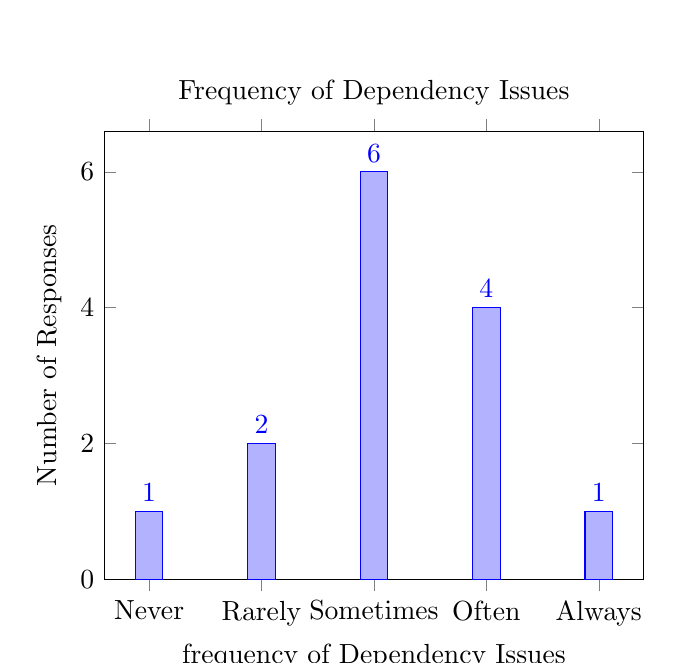
\begin{tikzpicture}
		\begin{axis}[
				ybar,
				symbolic x coords={Never, Rarely, Sometimes, Often, Always},
				xtick=data,
				nodes near coords,
				ymin=0,
				ylabel={Number of Responses},
				xlabel={frequency of Dependency Issues},
				title={Frequency of Dependency Issues}
			]
			\addplot coordinates {(Never,1) (Rarely,2) (Sometimes,6) (Often,4) (Always,1)};
		\end{axis}
	\end{tikzpicture}
	\caption{Frequency of Dependency Issues encountered by respondents}
	\label{fig:frequency}
\end{figure}

Respondents reported using a variety of tools for their dependency management needs, most commonly npm (8), Maven (5), and Gradle (4). Other tools that were used were pip (3), and 1 of each Bundler, Conan, and Composer. This shows that there is a diverse range of dependency management tools used, each with some similiar features but other things that they are missing.

\begin{figure}[ht]
	\centering
	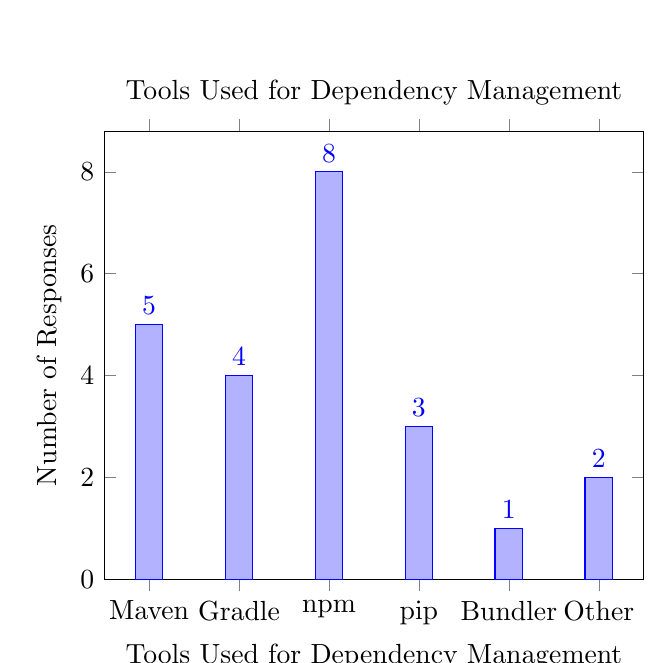
\begin{tikzpicture}
		\begin{axis}[
				ybar,
				symbolic x coords={Maven, Gradle, npm, pip, Bundler, Other},
				xtick=data,
				nodes near coords,
				ymin=0,
				ylabel={Number of Responses},
				xlabel={Tools Used for Dependency Management},
				title={Tools Used for Dependency Management}
			]
			\addplot coordinates {(Maven,5) (Gradle,4) (npm,8) (pip,3) (Bundler,1) (Other,2)};
		\end{axis}
	\end{tikzpicture}
	\caption{Tools Used for Dependency Management by respondents}
	\label{fig:tools}
\end{figure}

Satisfaction rates varied significantly, with 3 respondents very satisfied with their current solution, 5 satisfied, 4 relatively neutral, 2 report dissatisfaction. No respondents indicated that they were extremely dissatisfied with their package manager. These results help to show that respondents are generally satisfied with their dependency management solutions. However, there are still a significant proportion of developers who indicate that they are dissatisfied with the current state of software available, showing a continued need for improvement.

The most significant challenges that were faced in version conflicts (9), security vulnerabilities (6), compatibility issues (5), and lack of documentation (4). Other challenges that some respondents listed were licensing issues and network latency issues. Version conflicts emerged as the predominant issue, highlighting the need for managing them.

\begin{figure}[ht]
	\centering
	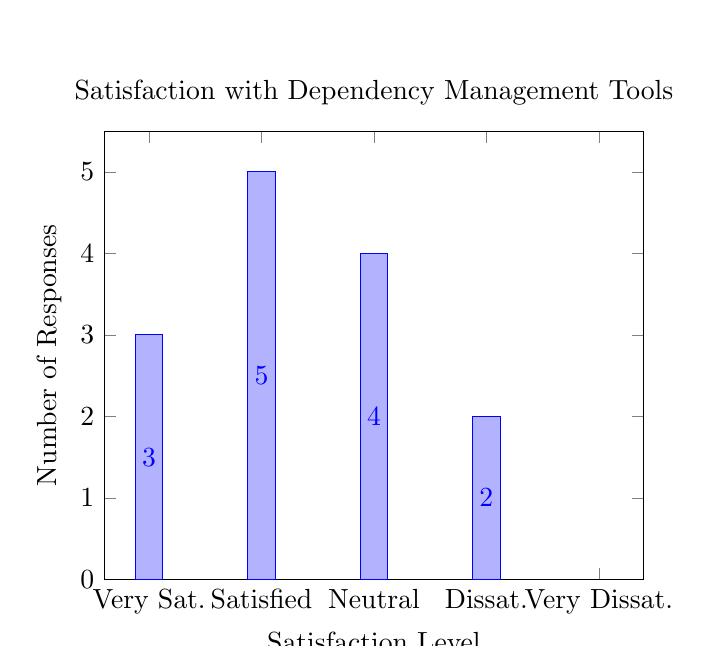
\begin{tikzpicture}
		\begin{axis}[
				ybar stacked,
				symbolic x coords={Very Sat., Satisfied, Neutral, Dissat., Very Dissat.},
				xtick=data,
				nodes near coords,
				ymin=0,
				ylabel={Number of Responses},
				xlabel={Satisfaction Level},
				title={Satisfaction with Dependency Management Tools}
			]
			\addplot coordinates {(Very Sat.,3) (Satisfied,5) (Neutral,4) (Dissat.,2) (Very Dissat.,0)};
		\end{axis}
	\end{tikzpicture}
	\caption{Satisfaction with Dependency Management Tools}
	\label{fig:satisfaction}
\end{figure}

Luckily developers considered dependency management an important issue with the majority considering it important (6) or extremely important (4). There was one respondent who noted it was slightly important, and no one noted dependency management as completely unimportant. The vast majority (10) indicated that they felt a greater degree of training and resources in dependency management would be useful.

\begin{figure}[ht]
	\centering
	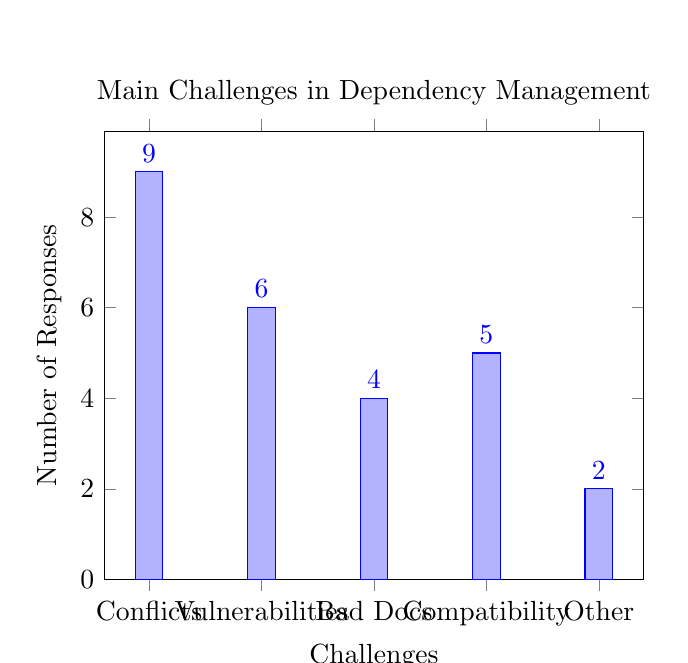
\begin{tikzpicture}
		\begin{axis}[
				ybar,
				symbolic x coords={Conflicts,  Vulnerabilities, Bad Docs, Compatibility, Other},
				xtick=data,
				nodes near coords,
				ymin=0,
				ylabel={Number of Responses},
				xlabel={Challenges},
				title={Main Challenges in Dependency Management}
			]
			\addplot coordinates {(Conflicts,9) (Vulnerabilities,6) (Bad Docs,4) (Compatibility,5) (Other,2)};
		\end{axis}
	\end{tikzpicture}
	\caption{Main Challenges in Dependency Management faced by respondents}
	\label{fig:challenges}
\end{figure}

Overall, the survey results show that dependency management is still a considerable issue within the software development industry. Version conflicts, security vulnerabilities, and compatibility issues are the major areas within dependency management where many users see issues. There is a clear need for more effective dependency management software, and multiple respondents indicated that they would appreciate a more standardized approach between different languages. The fact that many developers are currently relying on manual updating shows that further automatic dependency management features would be helpful.

\section{Related Work}
Serverless computing has been extensively studied in recent years, with a particular focus on its scalability, cost-effectiveness, and ease of deployment. However, the security implications of dependency management in serverless environments have received comparatively less attention. This section reviews the key contributions of existing studies and identifies the gaps that our research aims to fill.

\textbf{Security Challenges in Serverless Computing}

Baldini et al. (2017) provide a foundational understanding of the security challenges in serverless architectures. They highlight the inherent vulnerabilities introduced by the use of third-party libraries and the difficulties in maintaining secure environments without traditional server management. Similarly, Roberts et al. (2020) emphasize the shift in developer responsibilities towards code maintenance and dependency management, underlining the need for automated tools to handle these tasks efficiently.

Our work builds on these foundational studies by focusing specifically on the role of automated dependency management tools, such as Snyk and Dependabot, in mitigating security risks. While previous research has identified the security challenges, our study provides a detailed evaluation of the tools designed to address these challenges, offering practical insights into their effectiveness and limitations.

\textbf{Automated Dependency Management}

Hilton et al. (2016) discuss the benefits of continuous integration (CI) and automated testing in software development, noting that automated dependency management can significantly reduce the manual effort required to maintain secure and up-to-date libraries. However, their study does not delve into the specifics of how these tools perform in serverless environments.

Marin et al. (2022) explore the security risks associated with dependency management in serverless applications, noting the importance of automated tools in mitigating these risks. Their research provides a broad overview but lacks a focused analysis of specific tools and their real-world applications.

Our research addresses this gap by conducting a focused examination of popular tools like Snyk and Dependabot, assessing their performance in real-world serverless applications. Through an online survey of developers, we gather practical insights and perceptions, which complement the technical evaluations found in previous studies. This dual approach allows us to provide a comprehensive understanding of both the technical and practical aspects of automated dependency management in serverless environments.

\textbf{Comparative Analysis of Serverless Platforms}

Several studies have compared the general features and performance of serverless platforms. Villamizar et al. (2015) provide a comparative analysis of AWS Lambda, Google Cloud Functions, and Azure Functions, focusing on their performance and scalability. While their study offers valuable insights into the capabilities of these platforms, it does not specifically address their dependency management features.

Our research adds a new dimension to the existing literature by examining the dependency management capabilities of these platforms in detail. We assess how AWS Lambda, Google Cloud Functions, and Azure Functions handle dependency management, including their integration with automated tools and the security features they offer. This detailed assessment is crucial for enhancing the security and reliability of serverless applications.
Practical Insights and Developer Perspectives

Previous studies have primarily focused on the technical aspects of dependency management and serverless computing. However, there is a lack of research on the practical challenges and perceptions of developers using these tools. Our online survey of developers provides valuable insights into the real-world practices and experiences of those working with serverless applications. By incorporating these perspectives, our research offers a more holistic view of the current state of dependency management in serverless environments.
Advancements and Future Directions

Our work advances the field by identifying specific areas for improvement in automated dependency management, such as enhanced vulnerability scanning, better transparency in automated updates, and increased developer education. These recommendations are based on our detailed analysis and survey findings, offering practical solutions to the challenges identified in previous studies.

In conclusion, while existing research has laid the groundwork for understanding the security challenges and benefits of automated dependency management in serverless computing, our study provides a focused and detailed analysis of specific tools and platforms. By filling the gaps in the current literature and offering practical insights, our research contributes to the ongoing efforts to enhance the security and efficiency of serverless applications.


\section{Conclusion}

As serverless computing continues to evolve, the automation of dependency management emerges as a critical factor in maintaining the security and stability of serverless applications. This paper has provided a comprehensive analysis of automatic dependency management tools and practices in serverless environments, focusing on the security implications associated with these practices.

Our comparative analysis of AWS Lambda, Google Cloud Functions, and Azure Functions reveals that each platform offers unique strengths and weaknesses in handling dependency management and security. AWS Lambda excels in its robust ecosystem and extensive community support, making it a reliable choice for developers seeking comprehensive security features and seamless integration with various tools. Google Cloud Functions stands out for its user-friendly interface and strong performance, supported by comprehensive documentation and robust security features. Azure Functions offers enterprise-grade support and highly customizable environments, making it an ideal choice for organizations with complex security requirements and a need for strong performance and reliability.

Despite the advancements in automatic dependency management, challenges remain. Issues such as performance impact, compatibility, and the risk of vendor lock-in must be carefully managed. The survey of developers highlighted the ongoing need for improved tools and practices, emphasizing the importance of continuous monitoring, regular updates, and developer education.

In conclusion, while automatic dependency management significantly enhances the security of serverless applications, it is not a panacea. Developers must remain vigilant and proactive, leveraging the strengths of their chosen platforms while mitigating potential risks. As the serverless paradigm continues to grow, the development of more sophisticated and user-friendly dependency management tools will be crucial in ensuring the security and resilience of serverless applications.

Future research should focus on exploring new methods for improving the transparency and reliability of automatic dependency updates, as well as developing standardized best practices for dependency management across different serverless platforms. By addressing these challenges, the industry can continue to advance towards more secure and efficient serverless computing environments.

\bibliographystyle{ACM-Reference-Format}
\bibliography{references}

\end{document}